\chapter*{Dodatak: Prikaz aktivnosti grupe}
		\addcontentsline{toc}{chapter}{Dodatak: Prikaz aktivnosti grupe}
		
		\section*{Dnevnik sastajanja}
		
		\begin{packed_enum}
			\item  sastanak
			
			\item[] \begin{packed_item}
				\item Datum: 16. listopada 2023.
				\item Prisustvovali: svi članovi grupe
				\item Teme sastanka:
				\begin{packed_item}
					\item dogovor oko korištenih tehnologija
					\item okvirna podjela na podtimove
				\end{packed_item}
			\end{packed_item}
			
			\item sastanak
			
			\item[] \begin{packed_item}
				\item Datum: 20. listopada 2023.
				\item Prisustvovali: Božo Đerek, Lucija Lovrić
				\item Teme sastanka:
				\begin{packed_item}
					\item razrada plana i podjela posla za \textit{Opis projektnog zadatka}
				\end{packed_item}
			\end{packed_item}
		
			\item  sastanak
			
			\item[] \begin{packed_item}
				\item Datum: 25. listopada 2023.
				\item Prisustvovali: svi članovi grupe
				\item Teme sastanka:
				\begin{packed_item}
					\item razmatranje osmišljenog plana za bazu podataka
					\item izrada ER dijagrama
				\end{packed_item}
			\end{packed_item}
			
			\item sastanak
			
			\item[] \begin{packed_item}
				\item Datum: 30. listopada 2023.
				\item Prisustvovali: svi članovi grupe
				\item Teme sastanka:
				\begin{packed_item}
					\item razrada plana za \textit{Specifikaciju programske potpore}
					\item definiranje obrazaca uporabe
					\item definiranje ostalih zahtjeva
				\end{packed_item}
			\end{packed_item}
			
			\pagebreak
			
			\item sastanak
			
			\item[] \begin{packed_item}
				\item Datum: 31. listopada 2023.
				\item Prisustvovali: Lucija Runjić, Vedran Moškov, Andrija Merlin, Borna Josipović, Lana Bartolović
				\item Teme sastanka:
				\begin{packed_item}
					\item dogovor oko povezivanja \textit{back-end}-a s bazom podataka
				\end{packed_item}
			\end{packed_item}
			
			\item sastanak
			
			\item[] \begin{packed_item}
				\item Datum: 3. studenoga 2023.
				\item Prisustvovali: svi članovi grupe
				\item Teme sastanka:
				\begin{packed_item}
					\item dogovor oko \textit{Arhitekture i dizajna sustava}
				\end{packed_item}
			\end{packed_item}
			
			\item sastanak
			
			\item[] \begin{packed_item}
				\item Datum: 8. studenoga 2023.
				\item Prisustvovali: Lucija Runjić, Vedran Moškov, Borna Josipović, Andrija Merlin
				\item Teme sastanka:
				\begin{packed_item}
					\item izrada \textit{log-in} registra
					\item ostvarivanje potpune funkcionalnosti ruta za \textit{sign-up} i \textit{log-in}
				\end{packed_item}
			\end{packed_item}
			
			\item sastanak
			
			\item[] \begin{packed_item}
				\item Datum: 17. studenoga 2023.
				\item Prisustvovali: svi članovi grupe
				\item Teme sastanka:
				\begin{packed_item}
					\item revizija napravljenog
				\end{packed_item}
			\end{packed_item}
		
			\item sastanak
			
			\item[] \begin{packed_item}
				\item Datum: 7. prosinca 2023.
				\item Prisustvovali: svi članovi grupe
				\item Teme sastanka:
				\begin{packed_item}
					\item raspodjela posla i dogovor oko prepravljanja i punjenja baze podataka
				\end{packed_item}
			\end{packed_item}
			
			\item sastanak
			
			\item[] \begin{packed_item}
				\item Datum: 20. prosinca 2023.
				\item Prisustvovali: Lucija Runjić, Vedran Moškov, Borna Josipović, Andrija Merlin, Lana Bartolović
				\item Teme sastanka:
				\begin{packed_item}
					\item spajanje \textit{back-end}-a i \textit{front-end}-a za postavljanje novog oglasa i dodavanje komentara
				\end{packed_item}
			\end{packed_item}
			
			\item sastanak
			
			\item[] \begin{packed_item}
				\item Datum: 9. siječnja 2024.
				\item Prisustvovali: Lucija Runjić, Vedran Moškov, Borna Josipović, Andrija Merlin
				\item Teme sastanka:
				\begin{packed_item}
					\item dogovor oko stavljanja aplikacije na javni poslužitelj
				\end{packed_item}
			\end{packed_item}
			
			
			\item sastanak
			
			\item[] \begin{packed_item}
				\item Datum: 18. siječnja 2024.
				\item Prisustvovali: svi članovi grupe
				\item Teme sastanka:
				\begin{packed_item}
					\item revizija napravljenog
				\end{packed_item}
			\end{packed_item}
		\end{packed_enum}
		
		
		
		\eject
		\section*{Tablica aktivnosti}
			
			 \textit{Napomena: Doprinose u aktivnostima treba navesti u satima po članovima grupe po aktivnosti.}

			\begin{longtblr}[
					label=none,
				]{
					vlines,hlines,
					width = \textwidth,
					colspec={X[7, l]X[1, c]X[1, c]X[1, c]X[1, c]X[1, c]X[1, c]X[1, c]}, 
					vline{1} = {1}{text=\clap{}},
					hline{1} = {1}{text=\clap{}},
					rowhead = 1,
				} 
			
				\SetCell[c=1]{c}{} & \SetCell[c=1]{c}{\rotatebox{90}{\textbf{Andrija Merlin }}} & \SetCell[c=1]{c}{\rotatebox{90}{\textbf{Božo Đerek }}} &	\SetCell[c=1]{c}{\rotatebox{90}{\textbf{Lana Bartolović }}} & \SetCell[c=1]{c}{\rotatebox{90}{\textbf{Lucija Lovrić }}} &	\SetCell[c=1]{c}{\rotatebox{90}{\textbf{Vedran Moškov }}} & \SetCell[c=1]{c}{\rotatebox{90}{\textbf{Lucija Runjić }}} &	\SetCell[c=1]{c}{\rotatebox{90}{\textbf{Borna Josipović }}} \\  
				Upravljanje projektom 		& 2h  &  &  &  &  &  & \\ 
				Opis projektnog zadatka 	&  & 4h &  & 6h &  &  & \\ 
				Funkcionalni zahtjevi       &4h  & 6h &  & 6h &  &  & 3h \\ 
				Opis pojedinih obrazaca 	&  & 5h &  & 5h &  &  &  \\ 
				Dijagram obrazaca 			&  & 4h &  & 4h &  &  &  \\ 
				Sekvencijski dijagrami 		&  & 5h &  & 5h &  &  &  \\ 
				Opis ostalih zahtjeva 		&  & 1h &  &  &  &  &  \\ 
				Arhitektura i dizajn sustava	 & 2h  & 1h &  & 2h & 2h & 1h & 2h \\ 
				Baza podataka				&  & 3h & 4h &  &  & 5h &   \\ 
				Dijagram razreda 			&  & 11h & 4h &  &  &  &   \\ 
				Dijagram stanja				&  & 4h &  &  &  &  &  \\ 
				Dijagram aktivnosti 		&  & 2h &  &  &  &  &  \\ 
				Dijagram komponenti			&  & 2h &  &  &  &  &  \\ 
				Korištene tehnologije i alati 		&  & 1h &  & 3h  &  &  &  \\ 
				Ispitivanje programskog rješenja 	&   &  &  & 4h &  &  &  \\ 
				Dijagram razmještaja			&  & 1h &  &  &  &  &  \\ 
				Upute za puštanje u pogon 		& 2h & 2h &  &  &  &  &  \\  
				Dnevnik sastajanja 			&  &  &  & 1.5h &  &  &  \\ 
				Zaključak i budući rad 		&  &  &  & 3h  &  &  &  \\  
				Popis literature 			&  & 0.5h &  &  &  &  &  \\  
				&  &  &  &  &  &  &  \\ \hline 
				\textit{Frontend} 				&25h  &  & 74h &  &  &  & 87h \\  
				\textit{Izrada modela baze podataka} 		 			&  &  & 16h &  &  & 3h & \\  
				\textit{Spajanje s bazom podataka} 							&  &  &  &  & 11h & 7h &  \\ 
				\textit{Backend} 							&  &  &  &  & 56h & 60h &  \\ 
				\textit{Puštanje u pogon (deployment)} 							& 18h &  &  &  & 3h & 8h &  \\ 
				\textit{Testiranje rada aplikacije} 							& 2h &  &  &  & 8h & 10h & 7h \\ 
			\end{longtblr}
					
					
		\eject
		
		\section*{Dijagrami pregleda promjena}
		
		\begin{figure}[H]
			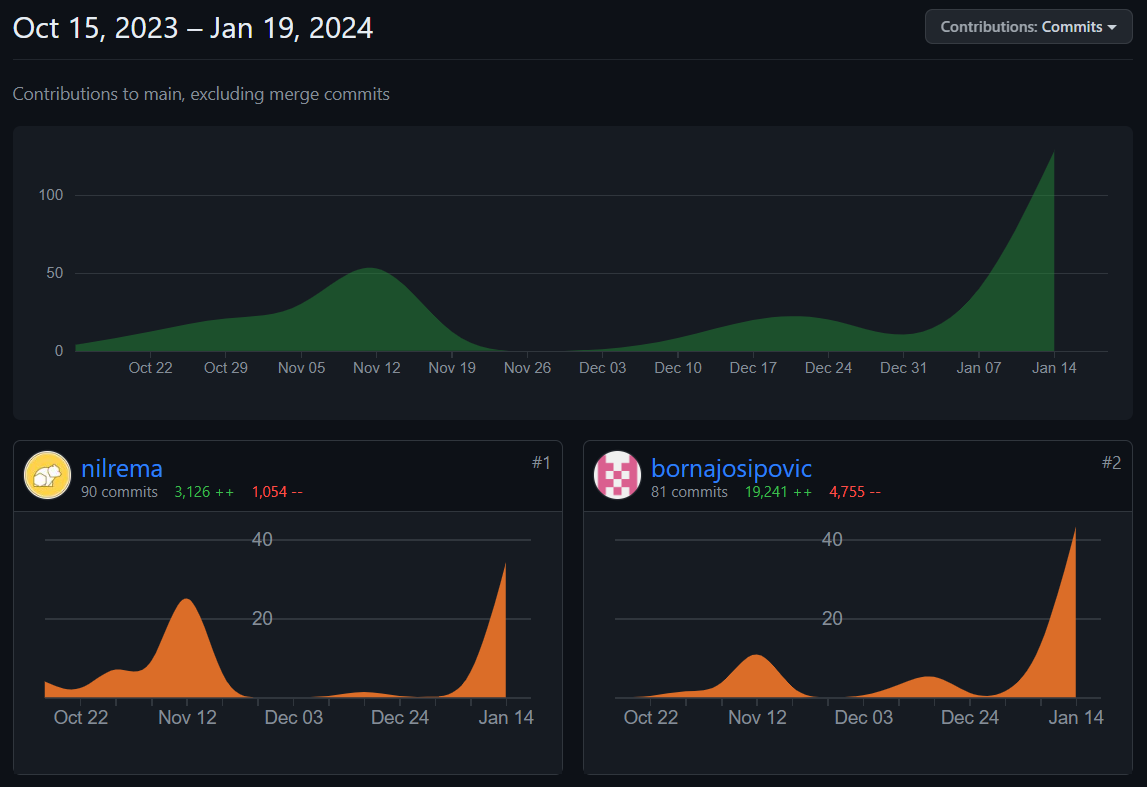
\includegraphics[scale=0.7]{slike/pregled_promjena_1.PNG} 
			\centering
			\caption{Pregled aktivnosti (1.)}
			\label{pregled_promjena_1}
		\end{figure}
		
		\begin{figure}[H]
			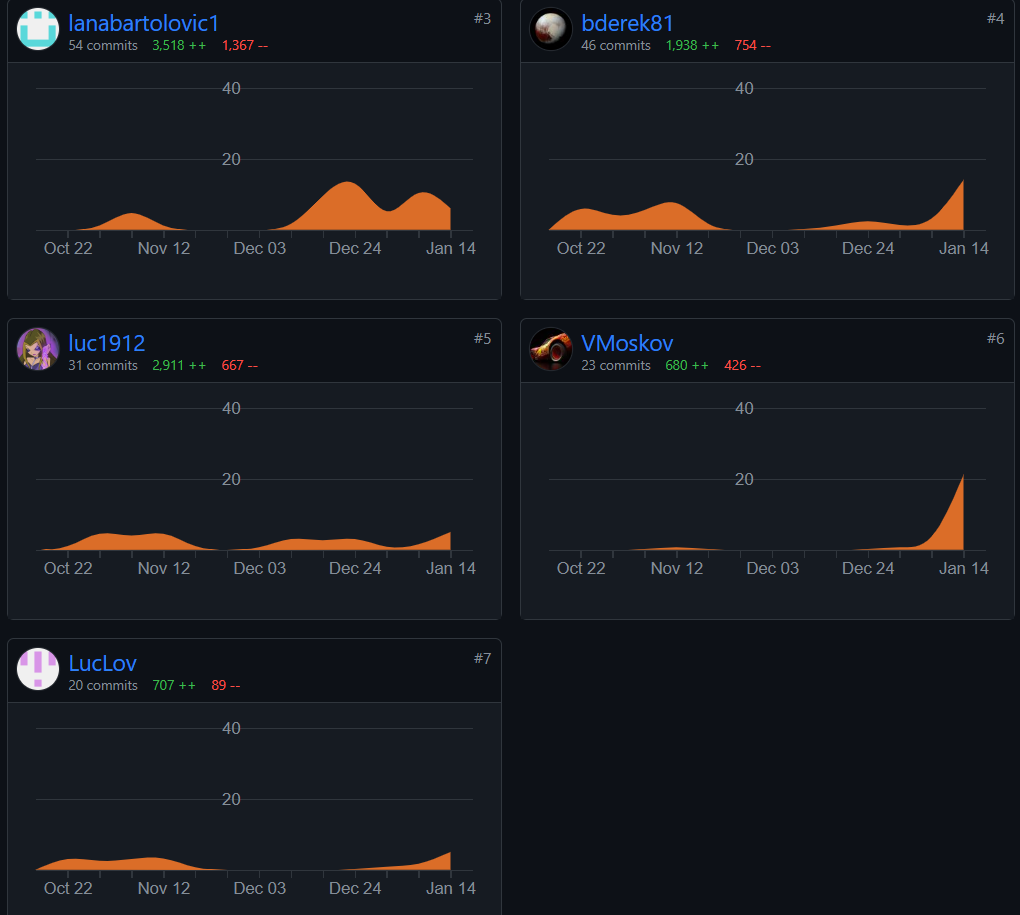
\includegraphics[scale=0.7]{slike/pregled_promjena_2.PNG} 
			\centering
			\caption{Pregled aktivnosti (2.)}
			\label{pregled_promjena_2}
		\end{figure}